\documentclass[fleqn,10pt]{wlscirep}
\title{Project on Surface Parameterization}

\author[1,*]{Xuan Li}
\affil[1]{Department of Computer Science, Stony Brook University}
\affil[*]{SBU ID: 111676019}

\newtheorem{definition}{Definition}[section]
\newtheorem{theorem}{Theorem}[section]
\newtheorem{corollary}{Corollary}[theorem]
\newtheorem{lemma}[theorem]{Lemma}


\usepackage{graphicx}
\usepackage{caption}
\usepackage{subcaption}

%\keywords{Keyword1, Keyword2, Keyword3}

\begin{abstract}
In this project, I implement three parametrization algorithms: Euclidean orbifold Tutte embedding \cite{Aigerman:2015:OTE:2816795.2818099}, hyperbolic orbifold Tutte embedding\cite{Aigerman:2016:HOT:2980179.2982412}, and boundary first flattening\cite{1704.06873}. The Euclidean orbifold Tutte embedding uses orbifold structure to generalize the algorithm in \cite{Gortler:2006:DOM:1133946.1648437} to sphere-type meshes. Hyperbolic orbifold Tutte embedding generalize the Euclidean orbifold Tutte embedding in the sense of geometry. But this generalization in non-linear. Besides, the Euclidean orbifold Tutte is also claimed to be conformal, so this algorithm provide a new linear method to compute conformal maps. Boundary first flattening is another linear conformal map solver. But this algorithm is based on differential geometry.
\end{abstract}
\begin{document}

\flushbottom
\maketitle
% * <john.hammersley@gmail.com> 2015-02-09T12:07:31.197Z:
%
%  Click the title above to edit the author information and abstract
%
\section{Theoretical Backgroud}
\subsection{Euclidean Orbifold Tutte Embedding}
The first part of my project is Euclidean orbifold Tutte embedding\cite{Aigerman:2015:OTE:2816795.2818099}. This algorithm is a generalization of so-called Tutte graph embedding based on the following theorem:
\begin{theorem}\label{tutte-theorem}
Let $G = \left<V , E , F \right>$ be a 3-connected planar graph with boundary vertices $B \subset V$ defining a unique unbounded exterior face $f_e$ . Suppose $\partial f_e$ is embedded in the plane as a (not necessarily strictly) convex planar polygon, and each interior vertex is positioned in the plane as a strictly convex combination of its neighbors, then the straight-line drawing of $G$ with these vertex positions is an embedding. In addition, this embedding has strictly convex interior faces.
\end{theorem}
The embedding problem is the following full-rank linear system:
\begin{equation}
\begin{split}
\sum_{v_j \in \mathit{N}(v_i)} w_{ij}x_j &= x_i, i = 1, ..., |V - B|\\
\sum_{v_j \in \mathit{N}(v_i)} w_{ij}y_j &= y_i, i = 1, ..., |V - B|\\
x_i &= b_i^x, i = |V-B| + 1, ... , |V|\\
y_i &= b_i^y, i = |V-B| + 1, ... , |V|
\end{split}
\label{eq:tutte}
\end{equation}
where $\sum_{j}w_{ij} = 1, \forall v_i$, and $w > 0$.
The result is guaranteed to be injective.

But this algorithm cannot be generalized onto topological sphere directly.
They \cite{Aigerman:2015:OTE:2816795.2818099} use a geometric structure called orbifold, making this method computable on sphere.

An orbifold can be treated as a tiled plane. The tile transformation is isometries. In this paper Euclidean orbifolds are used. We cut the mesh into disk to get a maximal submesh. The maximal submesh can be mapped to a tile of Euclidean plane. So besides Eq.\ref{eq:tutte}, we should make the embedding satisfy the following two conditions:

1. The embedding can tail the whole plane seamlessly.

2. The image of every vertex satisfy weighted convex combination on tiled plane.

For example, in Fig.\ref{fig:tile}, not only interior but also boundary vertices of the maximal submesh satisfy convex combination condition on the tiled plane.

\begin{figure}
\centering
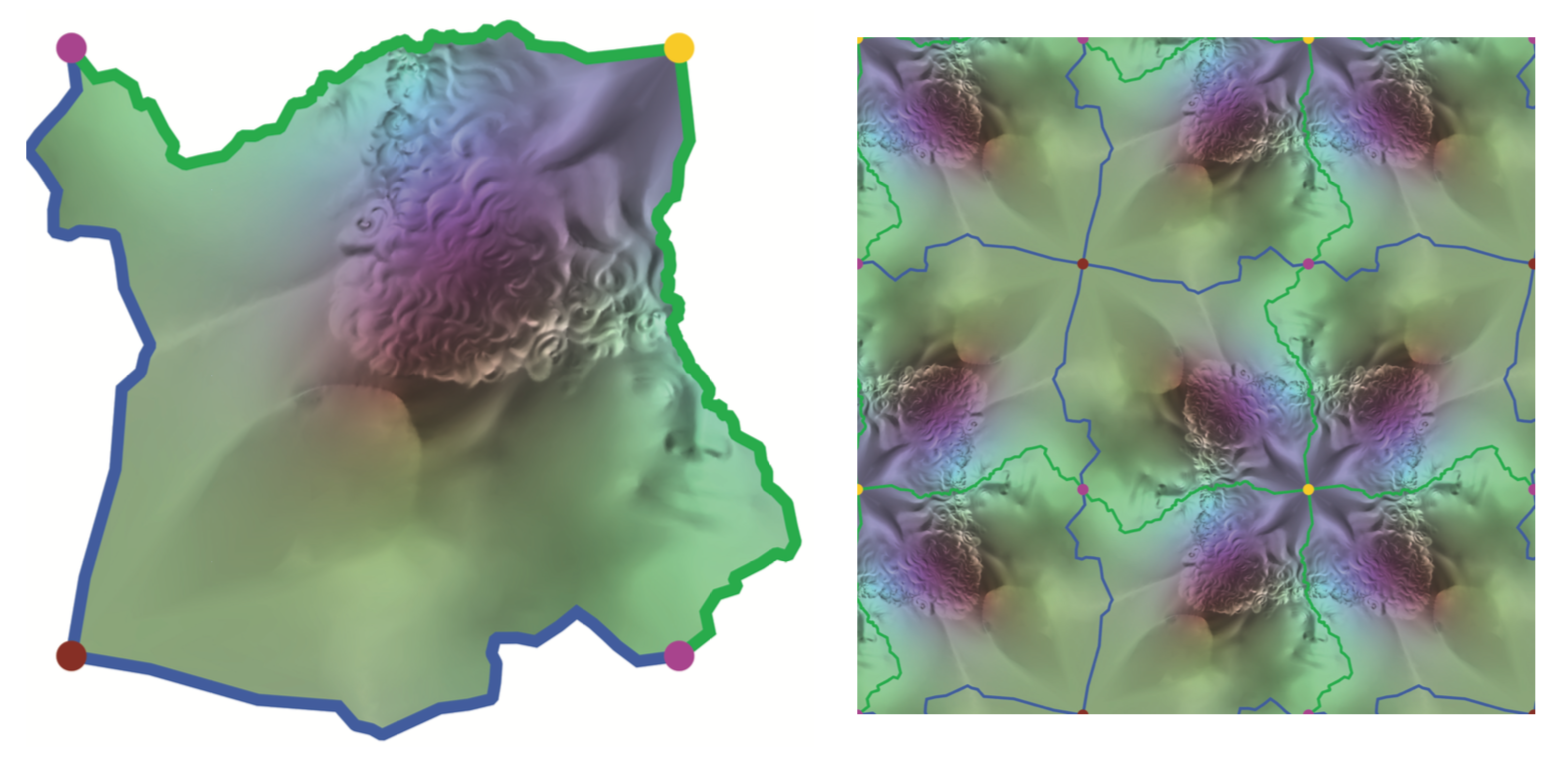
\includegraphics[width=0.5\textwidth]{images/euc_orbifold}
\caption{Tiled plane.}
\label{fig:tile}
\end{figure}

The system needs to be solved is:

\begin{equation}
\begin{split}
\sum_{v_j \in N(v_i)}w_{ij}(z_j - z_i) &= 0, &v_i \in \bar{V}-\bar{B}\\
\sum_{v_j \in N(v_i)}w_{ij}(z_j - z_i) + \sum_{v_j\in N(v_{i'})} w_{i'j}R_{i'i}(z_j - z_i')&= 0, &v_i \in \bar{B} - \bar{C}\\
z_i &= z_i^0 , &v_i \in \bar{C}
\end{split}
\end{equation}

Here we cut the $M$ into a submesh $\bar{M}$, which is a disk. $\bar{C}$ is the cones of the orbifold. $\bar{B}$ is
the boundary of the submesh. And $R_{i'i}$ is the rotation part of the isometry from $i'$ to $i$.

Note that we have only four Euclidean sphere-type orbifold, shown in Fig. \ref{fig:four-kinds}. And one intresting property is that the map is actually confomal map.

\begin{figure}
\centering
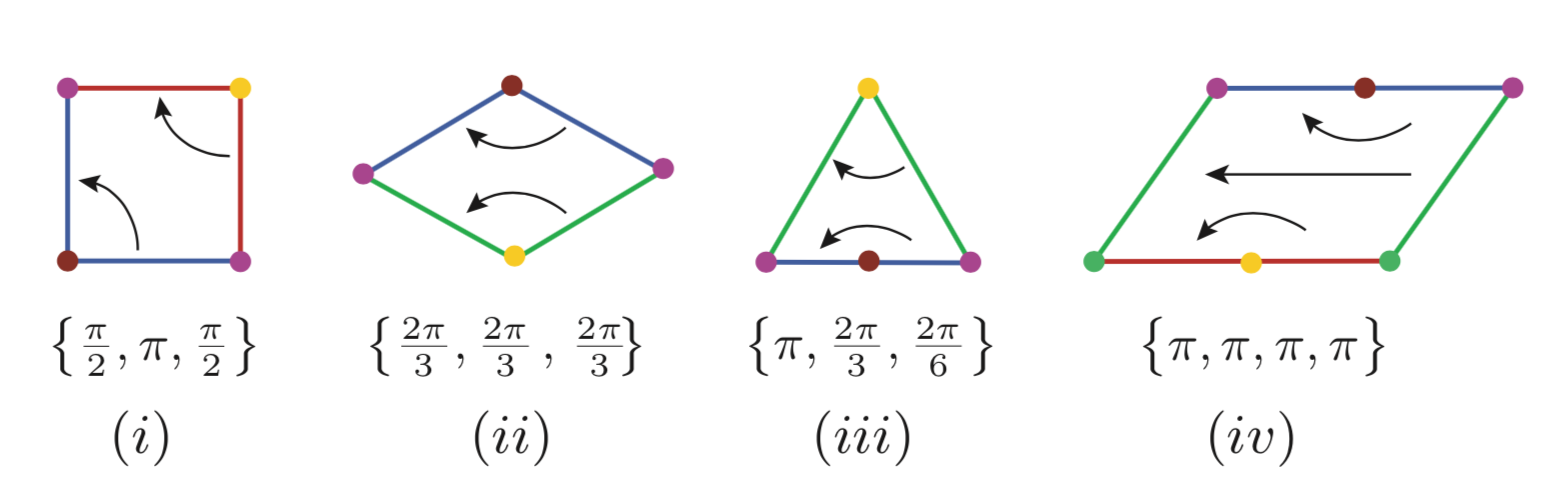
\includegraphics[width=0.5\textwidth]{images/four_euc_orbifolds}
\caption{Four kinds of sphere-type Euclidean orbifolds}
\label{fig:four-kinds}
\end{figure}


\subsection{Hyperbolic Orbifold Tutte Embedding}
The second part of my projects is hyperbolic orbifold Tutte embedding \cite{Aigerman:2016:HOT:2980179.2982412}. 
Hyperbolic orbifold Tutte embedding  is the generalization of Euclidean orbifold Tutte embedding. We treat a hyperbolic orbifold as a tiled Poincare disk by a basic tile. But hyperbolic isometries are non linear. Besides we use a non linear generalization of Tutte embedding:
\begin{equation}
\begin{split}
&\min_{\Phi}\ \ \   E(\Phi) = \frac{1}{2}\sum_{(i,j)\in E} w_{ij} d(z_i, z_j)^2 \\
s.t \ \ \   &z_i = z_i^0, \ \ \ \ v_i \in B
\end{split}
\end{equation}

where $d$ is the distance function in corresponding geometry. This system is equivalent to Eq.\ref{eq:tutte} in Euclidean geometry.

We use this generalization to get hyperbolic orbifolds:
\begin{equation}
\begin{split}
&\min_{\Phi} E(\Phi),&\\
s.t \ \ \ &z_i = m_{i'i}(z_{i'}), &v_i \in \bar{B} - \bar{C}\\
 &z_i = z_i^0, &v_i \in \bar{C}\\
\end{split}
\end{equation}
Here $d$ is hyperbolic distance function and $m_{i'i}$ is hyperbolic isometry from $i'$ to $i$.

The distance has explicit expression whose first order derivative is easily computed. So we can use first-order optimization algorithm to optimaize this problem.

A result from paper is showned in Fig.\ref{fig:hyper-orbifold} 

\begin{figure}
\centering
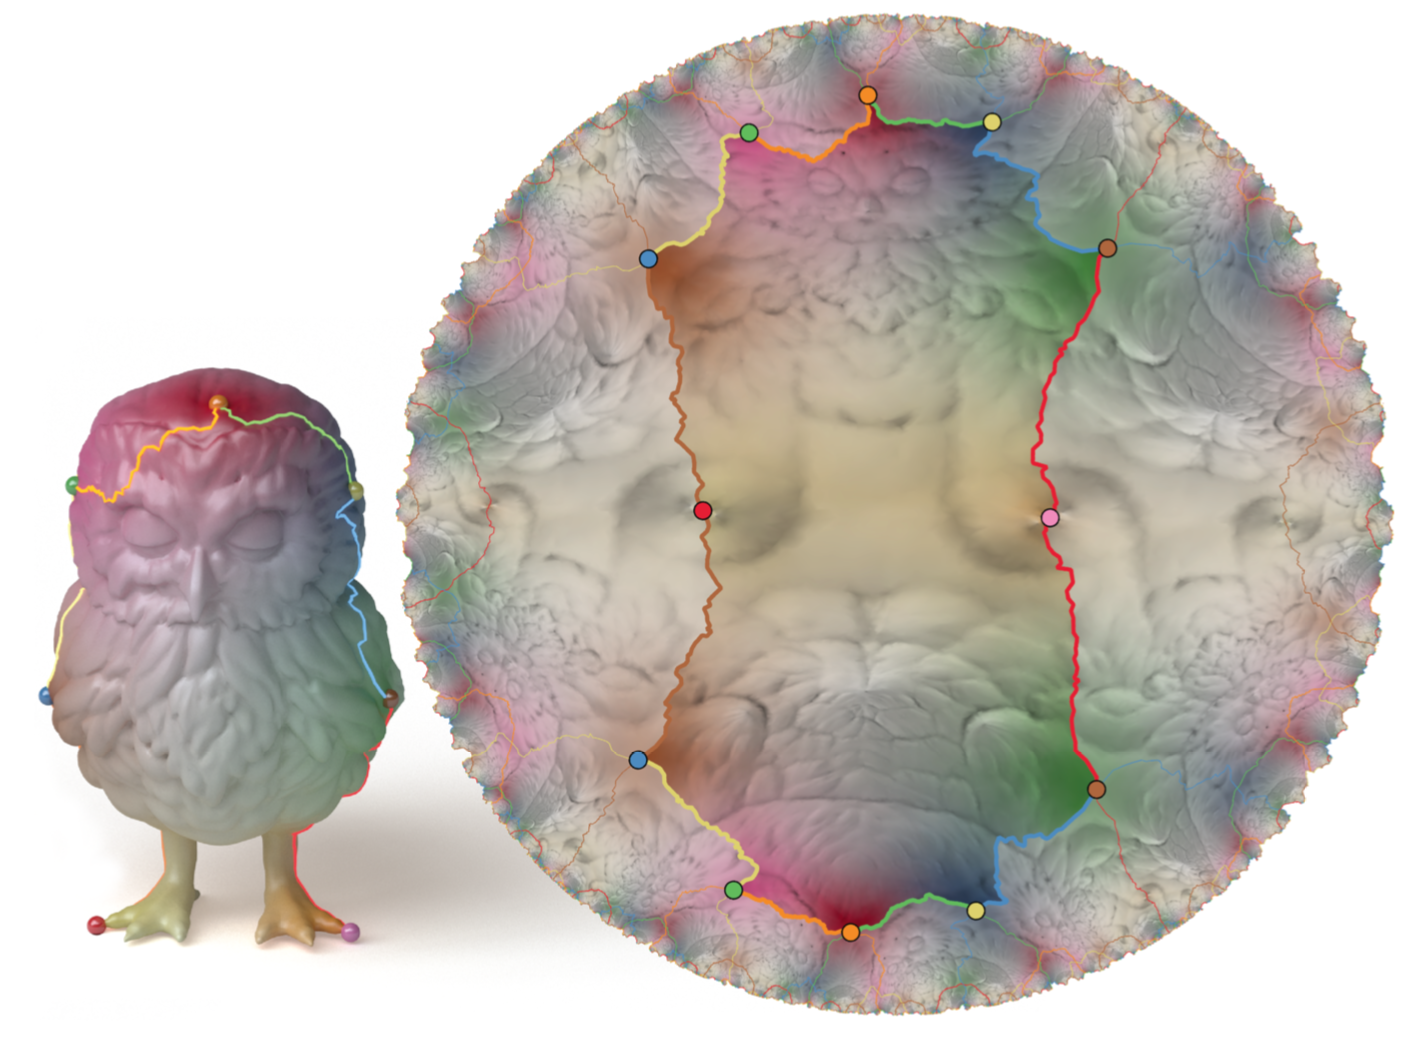
\includegraphics[width = 0.5\textwidth]{images/hyperbolic}
\caption{Hyperbolic orbifold Tutte embedding}
\label{fig:hyper-orbifold}
\end{figure}

\subsection{Boundary First Flattening}
The third part of my project is boundary first flattening \cite{1704.06873}. This is a linear method to compute a 






\section{Implementation Details}
\subsection{Overview}
\subsection{Dependencies}
\cite{eigenweb}\cite{libigl}\cite{LBFGSpp}\cite{Botsch02openmesh}


\section{Experiments}

 




\bibliographystyle{apalike}
\bibliography{sample}


\end{document}